\documentclass[tikz, varwidth=1600pt]{standalone}
\usepackage{amssymb, amsmath, bbm, graphicx}
\usetikzlibrary{positioning, arrows.meta} % Added arrows.meta for arrow connections

\begin{document}
\begin{tikzpicture}
    % Step 1 and Step 2
    \node[anchor=north west] (step1) at (0,0) {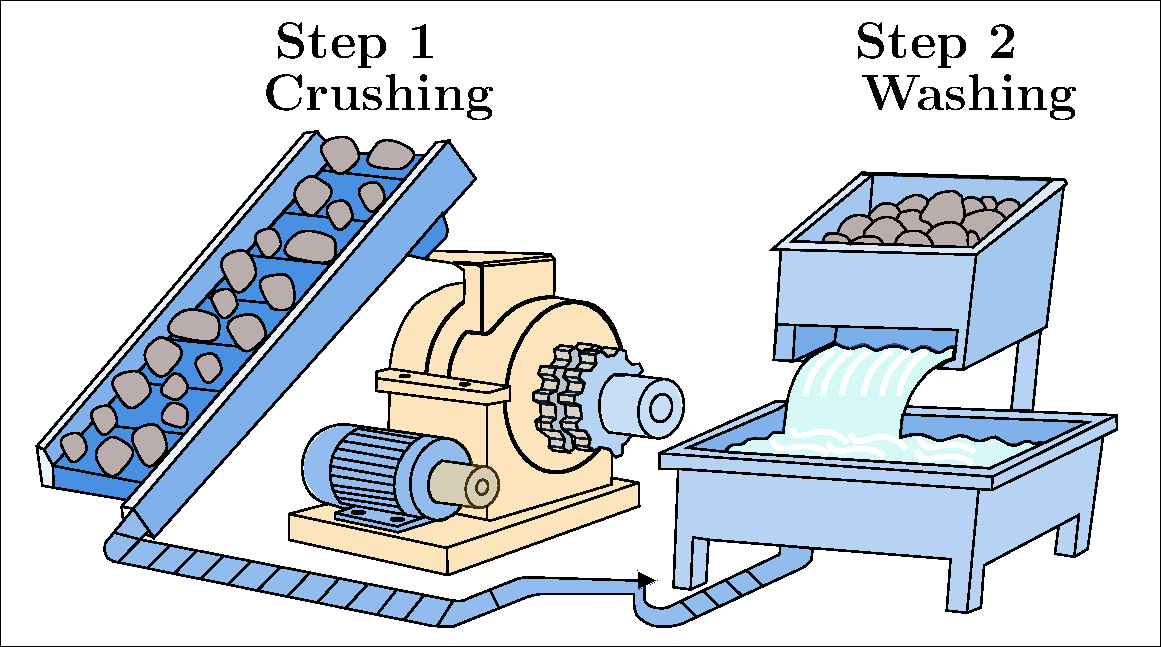
\includegraphics[width=5cm]{1and2}};

    % Step 3
    \node[right=of step1, xshift=1cm] (step3) {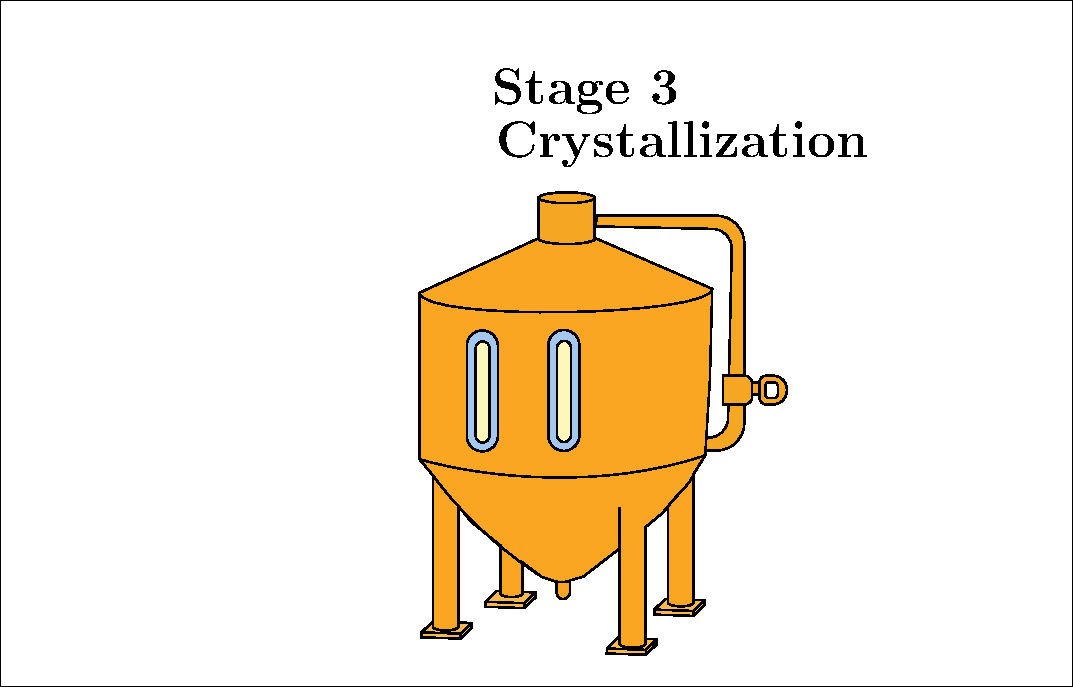
\includegraphics[width=5cm]{3}};

    % Arrow from Step 1 to Step 3
    \draw[->, thick] (step1.east) -- (step3.west);

    % Step 4
    \node[right=of step3, xshift=1cm] (step4) {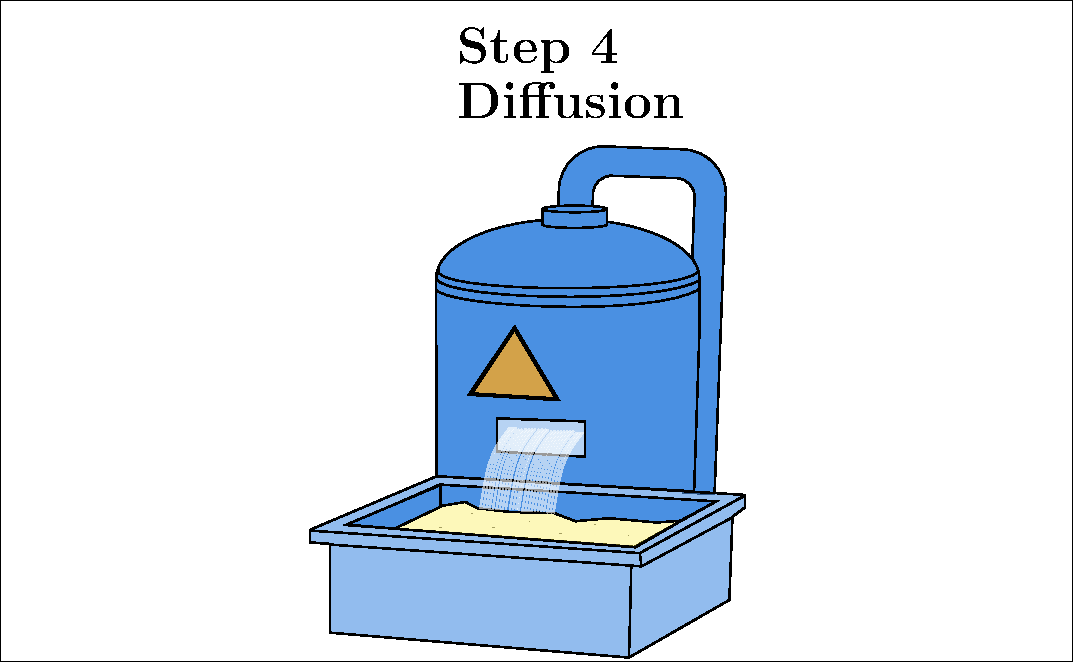
\includegraphics[width=5cm]{4}};

    % Arrow from Step 3 to Step 4
    \draw[->, thick] (step3.east) -- (step4.west);

    % Step 5 to the right of Step 4, but closer vertically
    \node[below=of step4, yshift=-0.5cm] (step5) {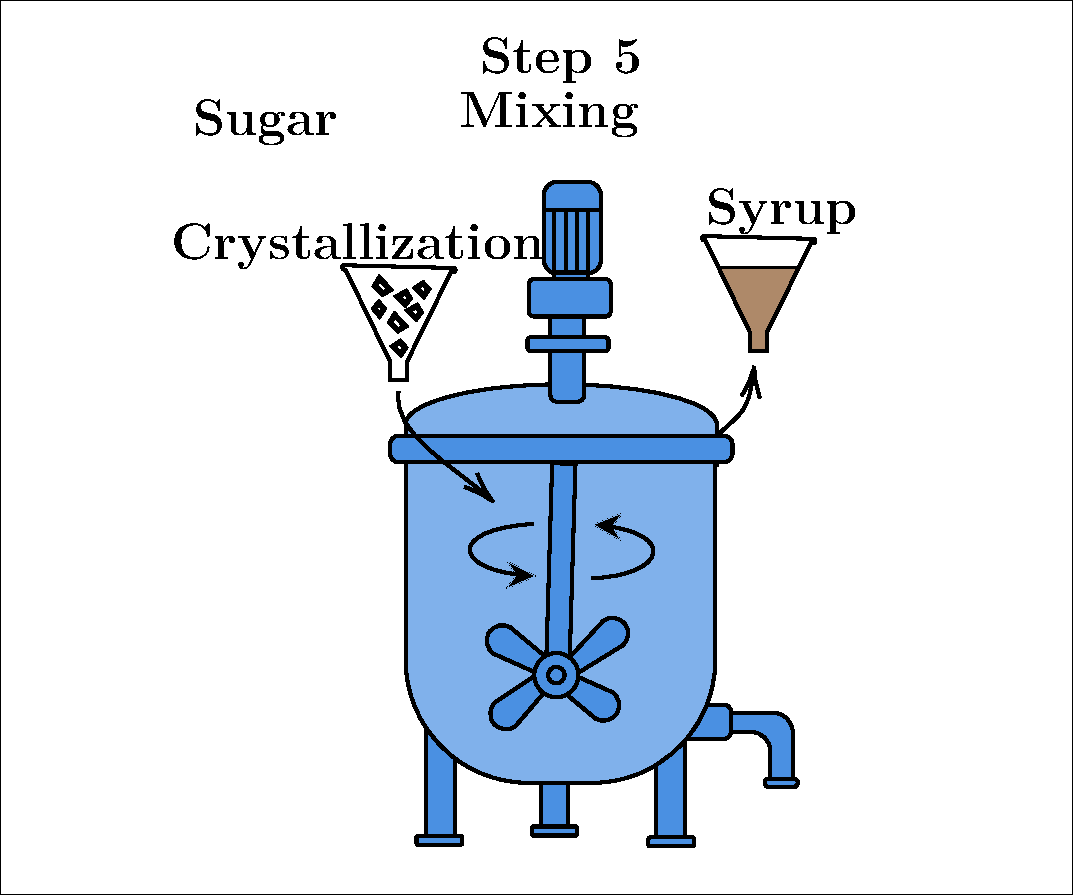
\includegraphics[width=5cm]{5}};

    % Arrow from Step 4 to Step 5 (short downward arrow)
    \draw[->, thick] (step4.south) -- (step5.north);

    % Step 6
    \node[left=of step5, xshift=-1cm] (step6) {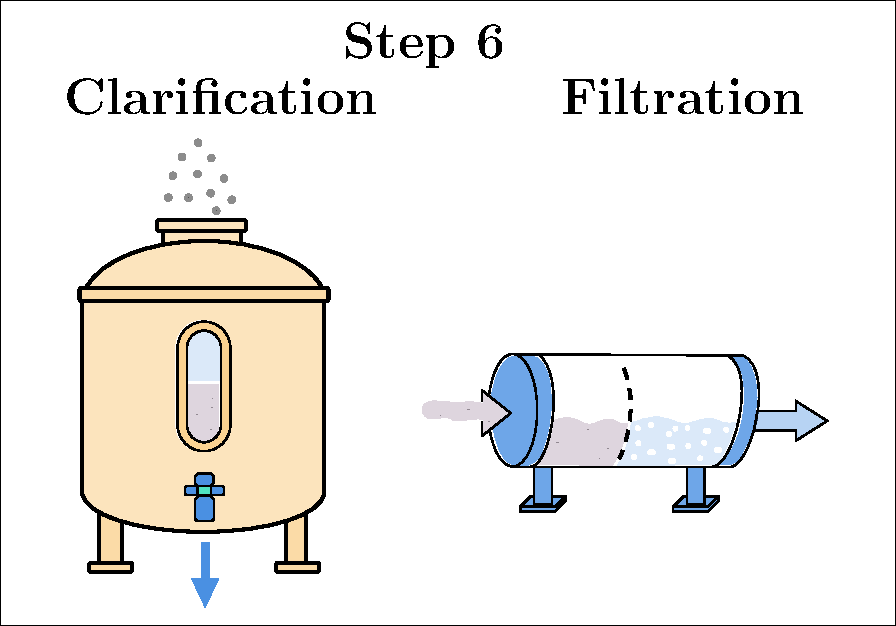
\includegraphics[width=5cm]{6}};

    % Arrow from Step 5 to Step 6
    \draw[->, thick] (step5.west) -- (step6.east);

    % Step 7
    \node[left=of step6, xshift=-1cm] (step7) {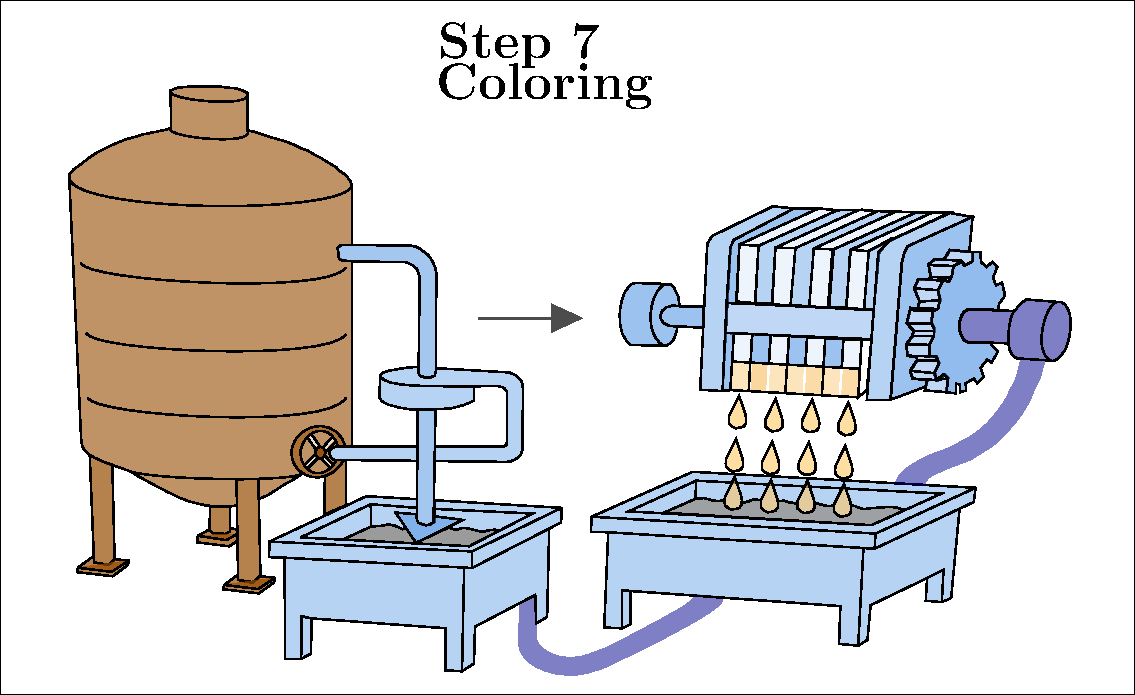
\includegraphics[width=5cm]{7}};

    % Arrow from Step 6 to Step 7
    \draw[->, thick] (step6.west) -- (step7.east);

    % Step 8
    \node[below=of step7, yshift=-0.5cm] (step8) {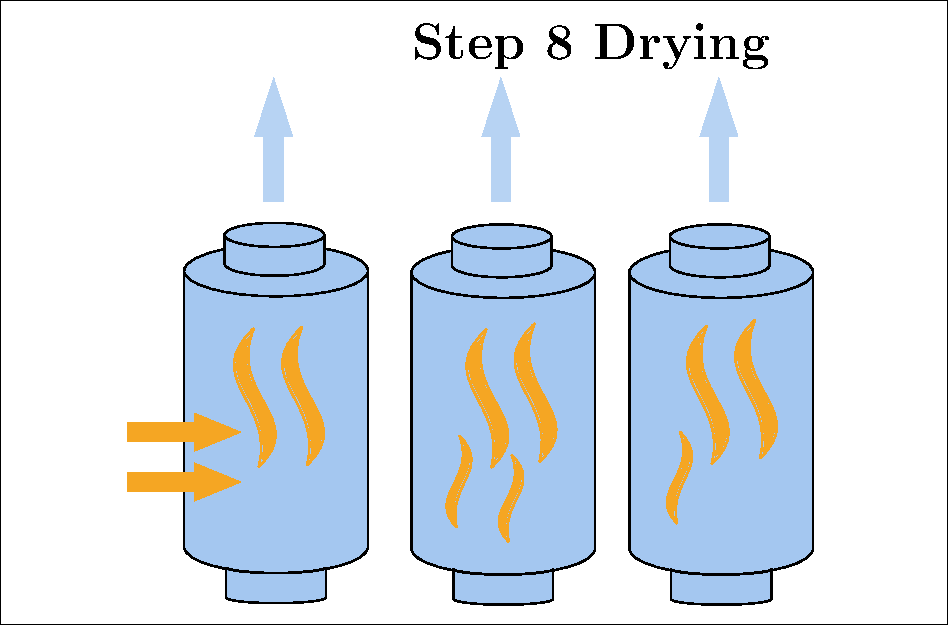
\includegraphics[width=5cm]{8}};

    % Arrow from Step 7 to Step 8 (short downward arrow)
    \draw[->, thick] (step7.south) -- (step8.north);

    % Step 9
    \node[right=of step8, xshift=1cm] (step9) {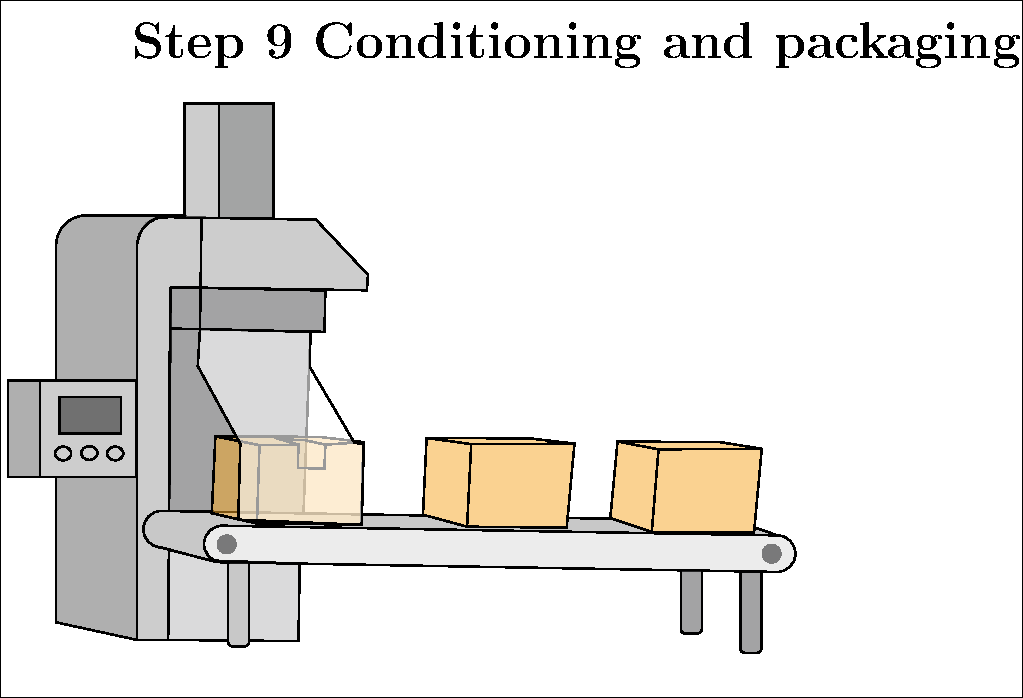
\includegraphics[width=5cm]{9}};

    % Arrow from Step 8 to Step 9
    \draw[->, thick] (step8.east) -- (step9.west);

    % Step 10
    \node[right=of step9, xshift=1cm] (step10) {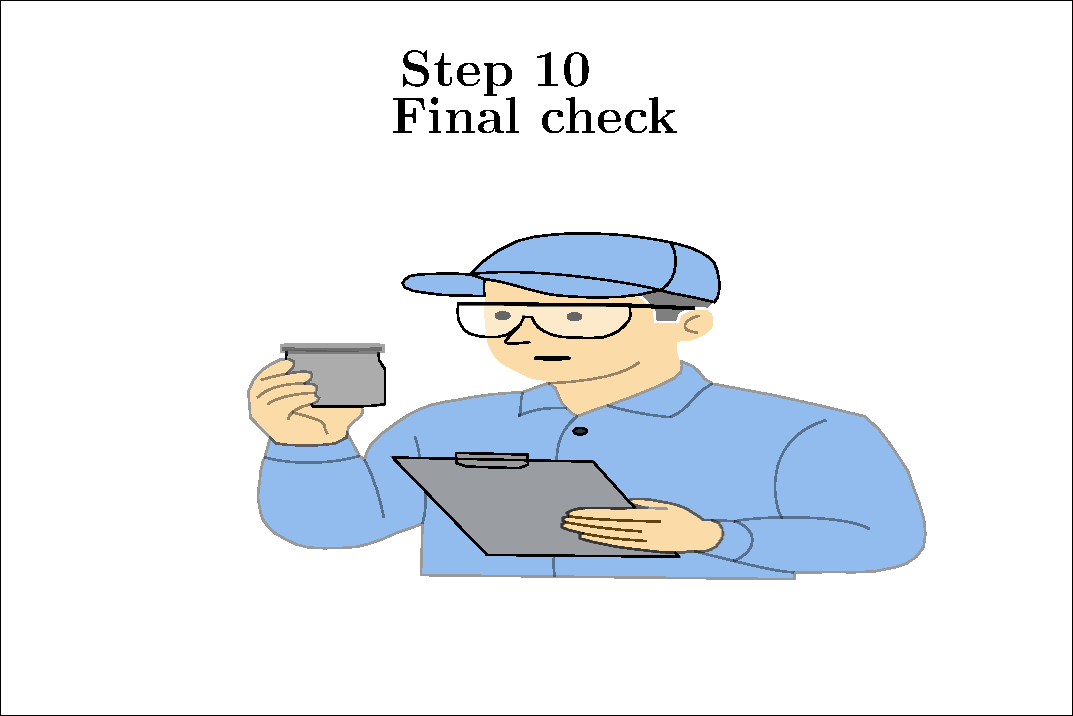
\includegraphics[width=5cm]{10}};

    % Arrow from Step 9 to Step 10
    \draw[->, thick] (step9.east) -- (step10.west);
\end{tikzpicture}
\end{document}